\documentclass{article}

\usepackage{newspaper}
\usepackage{times}
\usepackage{graphicx}
\usepackage{multicol}
\usepackage{caption}
\usepackage{wrapfig}
\usepackage{url}
\usepackage{picinpar}

\SetPaperName{NuWro News:}
\SetHeaderName{NuWro News}

\SetPaperLocation{
\includegraphics[width=80pt]{img/logo.png}}
\SetPaperSlogan{\vspace{-5pt}``You use Monte Carlo until you understand the problem.''\\\mbox{}\\ \hfill Mark Kac\vspace{-5pt}}

\SetPaperPrice{ebc7405}

\date{FEBRUARY 26, 2018}
\currentvolume{18}
\currentissue{2}

\begin{document}
\maketitle

\begin{center}
  {\vspace{5pt}\sc\huge NuWro 18.02 is now available!\vspace{5pt}}
\end{center}

\closearticle

{\Large\it This is an amazing news for the neutrino community. The NuWro collaboration has just announced the new release of their flag product. It is time to get excited! Lets see the most significant changes.}

\closearticle

\vspace{5pt}

\begin{minipage}{0.29\textwidth}

\vspace{10pt}

\headline{\it\bf\Large New NN cross sections}

It is the beginning of a revolution. The new framework for incorporating cross section data for nucleon-nucleon and pion-nucleon processes was introduced in the intranuclear cascade. It allows easily to update all re-interactions parameters to improve the model of final state interactions implemented in NuWro.

The NN scattering data from PDG was included in NuWro 18.02. On the top of that in-medium cross section modification from the Pandharipande-Pieper paper are introduced. The figure presents the nuclear transparency ratio of NuWro 18.02 prediction to experimental data for Carbon and Iron as a function of proton momentum. The agreement is superb! Shadowed bands correspond to experimental uncertainties.

\headline{\it\bf\Large Reweighting}

The first work on reweighting tools for NuWro was done by Luke Pickering and Patrick Stowell. Following their steps the NuWro team is including more and more knobs into the main code. Some new structures were introduced, some parts were rewritten from scratch. Long story short,~~ reweighting~~ is~~ included~~ in

\end{minipage}\hspace{0.5cm}\begin{minipage}{0.71\textwidth}

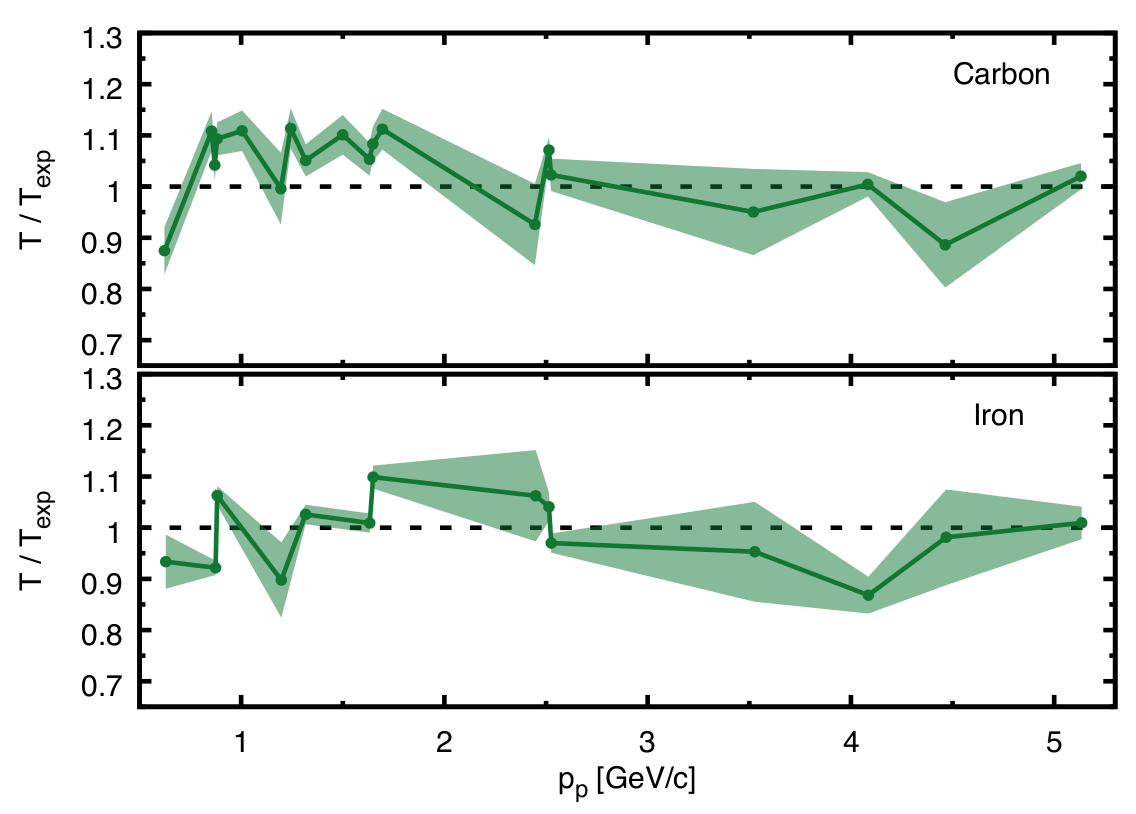
\includegraphics[width=0.9\textwidth]{img/1802_transparency.png}

\setlength{\linewidth}{0.9\textwidth}
\setlength{\columnsep}{0.5cm}

\begin{multicols}{2}{

NuWro 18.02. As everything in NuWro it is fast and user-friendly. As for today, the following parameters are available:

\begin{itemize}
 \item {\sc qel\_cc\_axial\_mass}
 \item {\sc qel\_nc\_axial\_mass}
 \item {\sc qel\_s\_axial\_mass}
 \item {\sc delta\_s}
 \item {\sc pion\_axial\_mass}
 \item {\sc pion\_c5a}
\end{itemize}

Please visit our user guide: \url{https://nuwro.github.io/user-guide/getting-started/parameters/} for their description.

\headline{\it\bf\Large Final remarks}

There are also some changes in default simulations parameters ({\sc params.txt}), e.g. final state interactions and Coulomb corrections for spectral function are now turned on by default. Some parameters are deprecated and replaced by new ones. New predefined beams and targets are available in new release.

The Singularity container (see \url{https://nuwro.github.io/user-guide/singularity/}) with NuWro 18.02 is available to make it easier for you to check the new release!

}\end{multicols}

\end{minipage}

\end{document}